\section{Distributed Implementations}
\label{implementation}

To handle extremely large graphs and large numbers of queries, we implement decentralized searches on a distributed general graph processing platform, Powergraph~\cite{180251}. As decentralized search has low online search space complexity and data dependencies upon each other, it is well suited to run multiple searches in a parallel way. 

\begin{figure*}[ht]
		\vspace{-0.7cm}
    \centering
    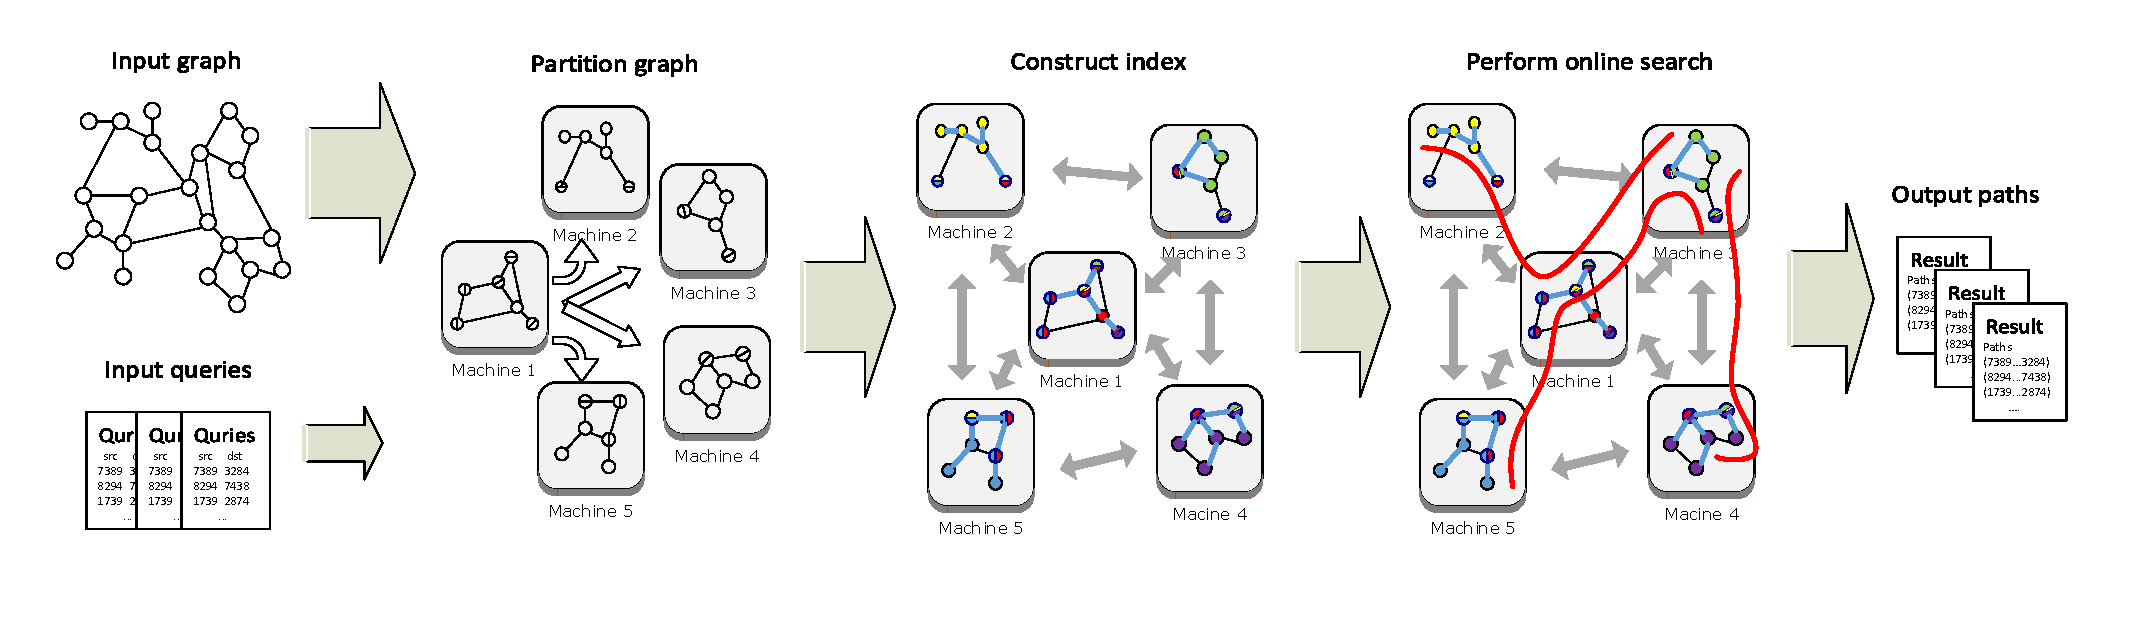
\includegraphics[width=\linewidth]{./figures/new_illustrate/system.pdf}
		\vspace{-1.2cm}
    \caption{A overview of distributed shortest path query processing system}
    \label{fig:system}
		\vspace{-2mm}
\end{figure*}

An overview of our shortest path query processing system is shown in Fig.~\ref{fig:system}. The system first use Powergraph to partition the graph onto multiple machines. Then several BFSs are performed to construct the index. After the index has been built, multiple shortest path queries can run in parallel. Large volumes of queries can submit repeatedly, for which responses will be generated at high throughput.

%\subsection{Decentralized search vertex-program}

Decentralized search can be implemented as vertex-programs in Gather-Apply-Scatter model used by Powergraph. Indexes are stored in a distributed way as vertex data. Each query instance contains the approximated path and the label of target vertex, as it is not accessible on each machine locally. Each step of decentralized search is split into Gather, Apply and Scatter phases. In the Gather phase, the LCA distance to the target vertex $d_{LCA}$ is collected from each neighbor and accumulated with a $sum$ function by finding the neighbor with the smallest $d_{LCA}$ as a next step candidate. In the Apply phase, the candidate is appended to the approximated path $\tilde{p}$ and the termination condition is checked. If it is met, the result path will be recorded and the query will be terminated. Otherwise, the program will proceed to the Scatter phase to start a new vertex-program on the candidate vertex and pass on the query instance. Algorithm~\ref{alg:vc_dec} shows the detailed algorithm.

\begin{algorithm}
    \caption{Decentralized search vertex program on $u$}
		\label{alg:vc_dec}
    \begin{algorithmic}
        \Function{gather}{$L(v), L(t)$} 
						\Comment {on neighbor vertex $v$}
						\State \Return $d_{LCA}(v, t)$, $v$
				\EndFunction

        \Function{sum}{$d_{LCA}(v_1,t)$, $v_1$, $d_{LCA}(v_2,t)$, $v_2$}
						\If {$d_{LCA}(v_1,t) \le d_{LCA}(v_2,t)$}
								\State \Return $d_{LCA}(v_1,t), v_1$
						\Else
								\State \Return $d_{LCA}(v_2,t), v_2$
						\EndIf
				\EndFunction

        \Function{apply}{$L(t)$, $\tilde{p}(s,t)$, $d_{LCA}(v,t)$}
						\If {$v \in L(t)$}
								\State $p_{remain} \gets$ path from $v$ to $t$ in $L(t)$
								\State append $p_{remain}$ to $\tilde{p}(s,t)$
								\State store $\tilde{p}(s,t)$
								\State $termination = true$
						\Else
								\State append $v$ to $\tilde{p}(s,t)$
								\State $termination = false$
						\EndIf
				\EndFunction

        \Function{scatter}{$L(t)$, $\tilde{p}(s,t)$, $termination$}
						\If {$\neg termination$}
								\State Activate($v$, $L(t)$, $\tilde{p}(s,t)$)
						\EndIf
        \EndFunction
    \end{algorithmic}
\end{algorithm}
The communication for the decentralized search happens during the Gather and the Scatter phase. In the Gather phase, the label of target vertex need to be passed to multiple machines, and the size is $O(k{\sigma}_{max})$. Each Gather function returns a $d_{LCA}$ along side of its id. Therefore, only $O(k{\sigma}_{max})$ size of data is transferred in total. In the Scatter phase, communication happens when activating the next step candidate. The whole search instance, including approximated path and label of target vertex, needs to be transmitted. The total size is $O(k{\sigma}_{max})$. Since the search will take as much as $2{\sigma}_{max}$ steps. So the overall communication overhead for each query is $O(k{{\sigma}_{max}}^2)$. 

During decentralized search, only the approximated path $\tilde{p}$ is updated at each step. Therefore, there is only $RAR$ type of data dependency among multiple decentralized searches on the underlying graph. Depending on implementations, there may be output dependency, i.e. $WAW$, when output $\tilde{p}$.

%The low memory and communication cost, along side with $RAR$-only data dependency during the search, makes a large number of decentralized search very suitable to run in parallel. To modify the vertex program for parallel processing, each vertex program maintains a list of search instances. Each query can be processed independently for all three phase which can achieve very high level of parallelism.
%During the Gather phase, the label of target vertex for each query is transmitted to other machines, and $d_{LCA}$ is calculated for each query. Query are updated during the Apply phase. In the Scatter phase, each query is examined for whether activating a certain vertex or not.
%
%\subsection{Distributed tie breaking strategy}
%%According to tie breaking strategy, multiple neighbors may be returned as candidates at the Gather phase. In this case, the search instance clones itself into multiple search instances and appends each candidate on each of the search instance at the Apply phase, and multiple searches are activated at the Scatter phase. 
%In our distributed implementation, the search instance clones itself into multiple search instances according to the tie breaking strategy. The problem is, as cloned search instances become independent in future steps, even one of them finds a shorter path than the others, it can hardly terminate other searches as such synchronizations are too costly in distributed environments. Therefore, a search may end up generating excessive number of child search instances. To overcome this problem, we pick one candidate at each step as a ``main'' candidate. For candidates that are not the ``main'' candidate, an extra termination condition is applied: In the following step, if the search cannot find a shorter path than expected, i.e. with a length shorter than $|\tilde{p}| + d_LCA$, the search will be discarded. 
%%The search space can be effectively controlled without compromise much accuracy.
%
%\subsection{Prune LCA computation}
%A major part of the computation overhead of decentralized search is large number of LCA computations. It is possible to prune the number of LCA computation required at each step for decentralized search to reduce the overall computation overhead. Suppose the search is visiting vertex $u$, then $d_{LCA}(u, t)$ has already been calculated in previous steps. If a neighbor vertex $v$ is a child of $u$ on the indexed shortest path tree $SPT_l$, then the LCA computation for $v$ and $t$ on $SPT_l$ does not need to be carried on as $d_{LCA_l}(v, t) > d_{LCA_l}(u, t)$. In practice, this principle can prune almost half of the total number of LCA computations of a search on average.
